\documentclass[10pt]{article}
\usepackage{common}
\usepackage{graphics}
\usepackage{graphicx}


\title{Multi-Document Text Summarization}
\author{Kevin Eskici (keskici@college.harvard.edu) \and Luis A. Perez (luis.perez.live@gmail.com)\\
Computer Science 182, Harvard University}
\begin{document}
\maketitle{}

\begin{abstract}
   We tackle the problem of multi-document extractive summarization by implementing two well-known algorithms for single-text summarization -- {\sc TextRank} and {\sc Grasshopper}.  We use ROUGE-1 and ROUGE-2 precision scores with the DUC 2004 Task 2 data set to measure the performance of these two algorithms, with optimized parameters as described in their respective papers ($\alpha =0.25$ and $\lambda=0.5$ for Grasshopper and $d=0.85$ for TextRank). We compare these modified algorithms to common baselines as well as non-naive, novel baselines and we present the resulting ROUGE-1 and ROUGE-2 recall scores. Subsequently, we implement two novel algorithms as extensions of {\sc GrassHopper} and {\sc TextRank}, each termed {\sc ModifiedGrassHopper} and {\sc ModifiedTextRank}. The modified algorithms intuitively attempt to ``maximize'' diversity across the summary. We present the resulting ROUGE scores. We expect that with further optimizations, this unsupervised approach to extractive text summarization will prove useful in practice.
\end{abstract}

\section{Introduction}
With an ever expanding amount of information available for consumption, automated processing of data into a human-readable format is of utmost importance. One approach to tackle this information overload involves  parsing sets of documents (imagine a series of news articles) and condensing them into the most important information that is nonetheless still consumable and interpretable by a human. The purpose of this paper is to propose and measure differing methods of reducing the cognitive overload imposed on individuals by the increasing amounts of available data.

Specifically, in this paper we seek to present two novel approaches to extractive corpus summarization. We tackle the problem of summarizing not a single sentence or a single document, but rather an entire body of work. The works must be topically related, and this assumption holds crucial in our exploration. With this in mind, the main goals of this paper and the related python packages are to:
\begin{itemize}
\item Understand current work in the field of automated text summarization.
\item Generalize the current work to a framework which incorporates expert knowledge about our current problem.
\item Compare two algorithms found in the literature, GrassHopper and TextRank, with current baselines as well as novel baselines.
\item Propose improvements to the above algorithms and implement them.
\item Evaluate all of the algorithms above using the ROUGE metric \cite{rouge}.
\item Create a usable library for text summarization in Python using the algorithms and baseline explored.
\end{itemize}

While the scope of the project is large, we are excited to report that we've addressed of all the above goals.\\

The system we developed is an all-encompassing and easy to use utility in Python that allows not only for summarization of arbitrary corpuses, but also provides an intuitive command-line interface for the summarization of arbitrary text. \\

For more details on how to work the program itself, see the latest updates found on the \href{https://github.com/kandluis/document_summaries}{github page}.

In this paper we now present the theoretical foundations behind the \verb|Summarizer|\footnote{The current name for our toy product!} library.

\section{Background}
Machine summarization of text lies at the cutting edge of natural language processing. Conferences such as the Document Understanding Conference (DUC) run large scale competitions on a yearly basis to push this frontier forward and encourage new development in algorithms for understanding text \footnote{For more information on these conferences, visit \href{http://duc.nist.gov/}{NIST}}. Two main methods are currently under study for summarization, an abstractive and extractive approach. Each method has its benefits and drawbacks, and while both are theoretically sounds, the current research tends to focus on extractive text summarization due to the inherent difficulty in building abstractive summarization models. We now discuss is approach in detail below.

\subsection{Abstractive Summarization}
The first approach is, theoretically, the most ideal. When given a document $d$ from some corpus $D$, intuitively, a summary seeks to capture the main ideas of the document. If we consider the document $d$ to consists of some general topics or ideas $T$ which are related through some set of relations $R$, abstractive summarizations seeks to ``understand'' the set $R$ extensively. It seeks not only to generate a summary, but generate a \textit{novel} summary by taking the collection of ideas $T$ and relating them in new, generalized ways leaned from the set of relations, $R$. While ideal, this approach has proved difficult to implement. \\

Currently, even summarization of a single sentence can take days to be computed as the system must understand not only the ``meaning'' of the sentence, but additionally, the grammatical structure underlying the language. Current research, such as that performed by Rush et al. \cite{rush_article}, has shown some improvements using some structurally simple models with large amounts of training data. However, even such extensive approaches with large amounts of training data which seek to generate new summaries tend to perform relatively poorly in the task of summarizing an entire document, $d$, and in particular, in the task of summarizing an entire corpus $D$. In fact, after thorough exploration of the literature, we have found no current research which seeks to accomplish this task as it appears to still be outside the scope of the AI community. \\

Systems that come the closes to even single sentence interpretations do exists, however, as has been demonstrated by  Le et al \cite{distributed_sentences}.

\subsection{Extractive Summarization}
Given the limitations of the theoretically preferable approach, an alternative has been developed which has shown to be relatively successful at both sentence  \cite{sentence_summary} and single document summarization. The idea behind this approach involves the following key insight: rather than learning the inherently difficult and complicated meaning of a sentence, we can make two simplifying assumptions in order to summarize a single document $d \in D$ where $D$ is our corpus of related documents.
\begin{enumerate}
\item Each sentence $s \in d$ represents a central, key idea.
\item Sentences in $s$ can be related through simple mathematical functions.
\end{enumerate}

The two simplifications above lead to extractive summarization. By (1), we now have a new sets of ``ideas'' $I$ given by:
$$
I = \{idea(s) \mid s \in d \}
$$

We can generalize the above to multi-document extractive summarization by presenting the set of ideas $I_D$ (the entire corpus) as simply the union of the set of ideas $I_d$ of each documents.
$$
I_D = \bigcup_{d \in D} I_d
$$

The second simplifications is also crucial in developing an extractive approach. This is because we can now relate each idea, which is in fact a vector sentence, to each other using what is termed similarity functions in the literature. If we think of each $idea(s) \in \mathbb{R}^n$, we can then seek to find a functions that allows for measuring similarity between sentences as simply functions that measure some property of two vectors. \\

In general, we can consider extractive sentence summarization as a ranking algorithm of sentences, where the purpose of a summarization algorithm is to select the best $k$ sentences given a single document $d$ in which $|d| > k$. In the abstract, this definition involves, crucially, accurately defining what is meant by ``best''. Current algorithms for extractive sentence summarization rely on defining ``best'' by looking at each sentence independently. The sentence with which most fully encapsulates the meaning of the body is then selected as a good candidate sentence. This algorithm is then repeated until the top $k$ sentences from our documents are selected.\\

However, even given the above generalizations of our definitions \footnote{Note that these definitions are in fact novel and have not been presented in the literature. However, throughout the development of our project, we found such abstractions and clear definitions of our objective helpful}, multi-Document extractive text summarization poses many unique challenges. While single document text summarization consists of selecting a good subset of sentences which summarize the document as a whole, with multi-document text summarization, we must consider a summary which not only does a good job of summarizing each document $d \in D$, but which can somehow incorporate the diversity of the entire set, $D$. Given the lack of available corpus data for training, extractive summarization on multi-document sets benefits from unsupervised, model-based approaches rather than supervised, data-driven methods. \\

\begin{algorithm}
  \begin{algorithmic}
    \Procedure{RankingSummarization}{$D, k$} //Where D is a set of documents and k is the length of the summary
    \State{$Results \leftarrow []$} \\ Intialize empty result set
    \While{$Results.len < k$}
      \State{$s \leftarrow \text{extractBest(D)}$} // Find the best sentence
        \State{$Results \leftarrow Results + [s]$} // Add to results set
    \EndWhile
  \State{$Summary \leftarrow sortSummary(Results)$}
    \EndProcedure{}
  \end{algorithmic}
  \caption{Simple Algorithm for Extractive Summarization}
\end{algorithm}

The above presents an introduction to the two main approaches for completing sentence summarization. Sentece summarization is an incredibly difficult task which requires precision, and even with extractive sentence summarization, we've run into our own set of challenges.

\section{Related Work}
As discussed in the background, we now dive into detail at some of the current work. Two main methods exists for current multi-document extractive summarization, each at a different stage of development.

\subsection{Summarization through Learning}
A simple approach which can be take to document summarization, where we consider only a single document $d$, is to train on previous data. Such an approach provides  a data-drive rather than model-driven approach to learning. We can, instead of generating a model of importance for the sentences or of appropriate summarization techiniques, simply look at existing data sets and existing summaries and attempt to learn patterns from the data. In particular, this approach has shown to be somewhat effective \cite{survey}. Of particular interest to our approach is the Hidden Markov Model of sentence extraction, as presented by Conroy an Dianne.

\subsubsection{Hidden Markov Models}
In \cite{hmm_summary}, Conroy and O'leary present a learning-based approach based on hidden markov models. The learning based approach uses training that that is, unsurprisingly, currently unavailable for download \footnote{This is a general complaint we have with the AI community which, for some reason, seems to refuse release their data or source code. We are of the opinion that researchers should follow our lead in releasing all utilized data, from start to end, as well as thorough instructions and source code focused on interpreting the results.}. \\

The main idea behind their model is to introduce a proabilisitic understanding to the idea of extractive sentence summarization. By looking through a data set of document-summaries pairs, they can calculate
$$
P(X_i \mid X_{i-1}), P(E_i \mid X_i)
$$
The first term is simply the transition probability of the system. Given that we have a previous sentence, what's the probability that the next sentence will also be contained in the summary? Conroy and O'leary discover, through their analysis, that the intuitive notion that sentences towards the beginning of are more important is in fact correct. The distributions tends to decay as the sentence moves further from the beginning, and this effects tends to be much larger for smaller summaries \footnote{While this is intuitively expected, it is good to have some data to back it up!} \cite{hmm_summary}. Furthermore, the result they present help inform us in the development of our own baselines, as we generate a system which uses this information directly. \\

With the above probabilities calculated (despite the lack of specification on the training data), the system could immediately be trained directly on the transition probabilities to generate a naive Bayesian approach. However, by utilizing an HMM, fewer assumptions on independence need to be made since the state $X_i$ learns all of the information about the states preceding it (or all of the relevant information). In particular, the largest benefit of the HMM is that it does not assume that the probability being in the summary is independent of the $i-1$ sentence being in the summary. \\

Intuitively, it makes sense to suppose that if a sentence is in th summary, sentence immediately following it would also be in the summary, likely dependent on the position of the sentences themselves. \\

Of particular interest is the feature representation used by the HMM, which mostly consist of the position of a sentence within its paragraph. Each sentence is assigned  a value $o_1(i)$ designating it as the first in the paragraph (value 1), the last in the paragraph (value $3$), or an intermediate sentence (value 2). \\

For a more thorough exposure to the details of the above, we propose seeing \cite{hmm_summary}. Here, we simply present the information relevant to informing our own approaches. In particualar, Figure \ref{fig:hmm_model} summarizer the approach relatively well.

\begin{figure}[h!]
\centering
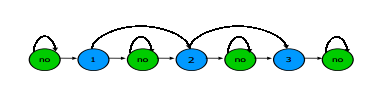
\includegraphics[]{hmm_model}
\caption{The HMM model recommended by \cite{hmm_summary}}.
\label{fig:hmm_model}
\end{figure}
There exist $2k+1$ states to the HMM which serve to indicate which sentences have been selected as we run over the paragraph to determine the results. \\

Of interest, we note that the paper by Conroy and O'leary also presents an alternative data-driven model approach which involves QR matrix factorization and latent variables \cite{hmm_summary}. For reference, it might be helpful to see \href{https://en.wikipedia.org/wiki/QR_decomposition}{Wikipedia} for some information on how QR decomposition of a matrix works. However, we find that such an approach is outside the scope of this paper and so defer to the reader the responsibility of understanding it.

\subsection{Summarization as Ranking - An Unsupervised Approach}
While the above approach appears promising, two main driving forces pushed us toward exploring a more unsupervised approach.
\begin{itemize}
\item The lack of available training data for extractive summaries. Automated methods (such as using Word's summary feature) are rather ineffective, and we'd rather compare to real human summaries.
\item The possibility of over-fitting on our training data. The purpose of our project includes creating a useable library, and given the diversity inherent to text, we felt it too likely that our results would prove fruitful only due to over-training and/or using test data too similar to our training data.
\end{itemize}

While each of the above is addressable in some way or other, and as shown by \cite{survey}, other have successfully addressed them, we take a different approach. Intead of admitting the limitations inherent to supervised summarization methods, we switch emphasis towards unsupervised learning methods.

In this scenario, we no longer require a set of data on which to train our model, instead utilizing the idea and algorithms presented in \cite{grasshopper} and \cite{textrank}. Both {\sc Grasshopper} and {\sc TextRank} are novel algorithms which take advantage of the grammatically and syntactical structure in inherent to text, and through expert knowledge, create summaries without requiring any training.

\subsection{Current Evaluation Methods}
However, we found that the evaluation of summaries presented by \cite{hmm_summary} was rather inadequate and it was not possible to recover their data. Therefore, taking such a supervised approach to the method of generating extractive summaries appeared less promising. Even other evaluation techniques, like those proposed in \cite{survey}, seemed somewhat arbitrary. \\

Rather than proposing subjective mechanisms similar to those mentioned above, we instead make use of a tool named ROUGE \cite{rouge}, developed for the explicit task of comparing summaries to one another. The tool, while widely used by DUC, appears to not have been used for either abstractive nor supervised extractive models \footnote{Obviously, this is given our limited research.}

\subsection{Multi-Document Summarization}
Current work specific to multi-document summarization is limited, though we did find two papers which discuss their algorithms in-depth, and which claimed competitiveness and effectiveness in the DUC 2004 competition \cite{grasshopper} \cite{textrank}.\\

In particular, note that these papers take an unsupervised approach to learning due to the exponential increase in data set diversity (with $n$ documents, there are a possible $2^n$ sets!

We therefore now detail the main changes we have made to tackle the issues faced when summarizing multiple documents. The changes reflect an increase need for “diversity” in the multi-document setting. We ignore words already included in our summaries when performing a search for the next candidate sentence. We also modify prior distributions to reflect knowledge on our document sets, creating multi-model priors over sentence selection. Furthermore, we make explicit modifications and propose novel algorithms for this work.

All changes are evaluated using an objective standard - ROUGE, specifically, ROUGE-R for the recall.

\section{Algorithms}
We implemented several baseline algorithms, most being original. The baselines follow one simple philosophy that we came across in our research which was to be simple and yet informative. Most of them follow the assumption that the distribution of sentence importance follows some type of exponential decay -- intuitively, the first few sentences are far more important that those towards the end. The inspiration for this follows \cite{hmm_summary}, as well as the general ideas presented in \cite{survey}, a survey of many summarization methods.

The main algorithms we implemented for this task were the graph based TextRank \cite{textrank} and GrassHopper \cite{grasshopper}. We further modified these algorithms in an attempt to improve their performance on the ROUGE-R metric, hoping to achieve results comparable to those of human summaries on multi-document sets.

\subsection{Baselines}
\subsubsection{Naive Baseline}
The simplest baseline involves taking the first $k$ sentences from the set of documents. This was the baseline from the DUC competition \footnote{\href{http://duc.nist.gov/duc2004/baseline_definitions}{Defintion of Baselines for DUC 2004 Competition}}. In fact, the baseline for the competition is more naive in that it takes only the first 665 characters of the latest document. In our implementation, we focus more on sentences extraction, so for a fair comparison, we extract the first $k$ sentences of the latest document.

\subsubsection{Geometric Prior}
This baseline is motivated by the idea that important sentences tend to appear at the beginning of articles as hinted at by the literature. After concatenating the documents into a single array of sentences, we choose a weighted random sample of sentences with weights proportional to the value of the Geometric PDF evaluated at a sentence's index. Recall that the Geometric distribution with parameter p has PDF:
$$ P(X = k) = (1- p)^x p$$
Figure \ref{fig:geom_prior} shows the pdf for several values of p. For our project we ended up using $p = 0.02$. We expect this parameter to be adequate for our purposes, though it is certainly true that it should be further optimized and tuned. In particular, Bayesian Optimization techniques look promising.

\begin{figure}[h!]
\centering
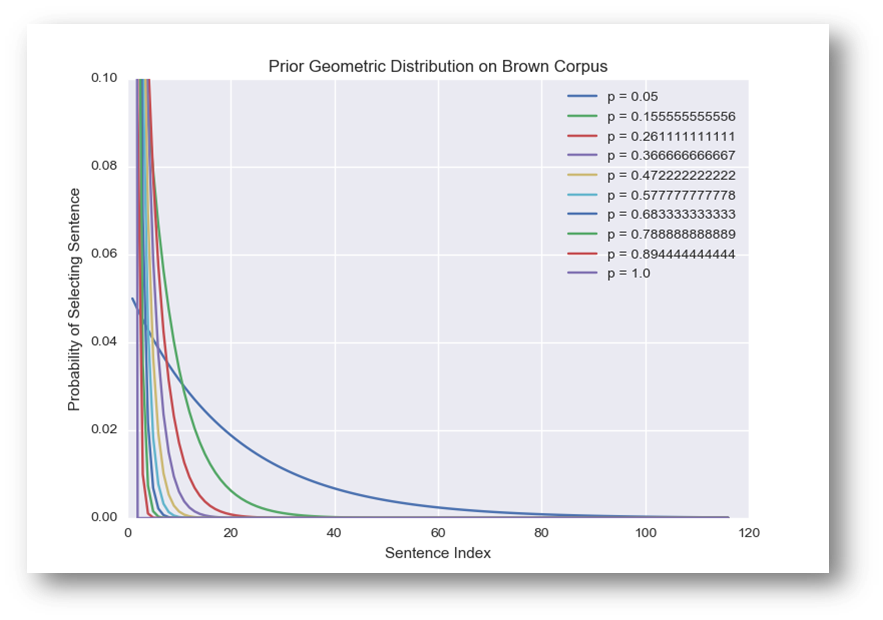
\includegraphics[scale=0.4]{geom_prior}
\caption{Plot of Geometric Prior for Different Values of $p$.}
\label{fig:geom_prior}
\end{figure}

\subsubsection{Modified Geometric Prior}
This approach tries to capture the benefits of the previous two by always taking the first sentence as part of the summary, and then randomly selecting the remaining $k-1$ sentences with weights determined by a Geometric distribution. We again used $p = 0.02$.

\subsubsection{Multiple Geometric Prior}
While reading the Geometric Prior section above, it may have seemed odd that sentence weights were proportional to the value of a Geometric PDF evaluated at a sentence's index in the array of concatenated sentences. If you thought "Wait a second, doesn't that mean the arbitrary ordering of documents will affect the weights?", you're right! Thus we implemented a Multiple Geometric Prior Baseline to account for this. The idea is simple-we assign each sentence a weight proportional to the value of the Geometric PDF evaluated at its corresponding index in it's OWN document. Then we re-normalize the vector of weights before drawing a weighted random sample of $k$ sentences.

\subsubsection{Word Frequency}
For our final baseline we decided to use a naive approach based on word frequency. After filtering out stop words, we go through the documents and count how many times each word appears in the concatenation of all documents in the set. After doing so, we use this mapping of words to frequencies to get sentence scores, where a sentences score is the sum of the scores of all words in the sentence, normalized by the length of the sentence. The sentence with the highest score is extracted as our fist summary sentence. Instead of simply taking the sentences with the next $k-1$ highest scores as the rest of the summary, we recompute sentence scores ignoring words already in our summary, take the sentence with the new highest score, and repeat until we have k sentences. This is done to avoid having the same words dominate our summary.

\subsection{TextRank}
After our baselines, we set out to apply the TextRank algorithm described in a paper by Mihalcea and Tarau \cite{textrank}. A graph algorithm, applying TextRank involve constructing an undirected network where sentences are vertices, and weighted edges are formed connecting sentences by a similarity metric.
We used the similarity function described in the paper, given below:
$$Sim(S_i, S_j) = \frac{| \{ w_k | w_k \in S_i \& w_k \in S_j\}|}{\log(|S_i|) + \log(|S_j|)}$$
After we have our graph, we can run the main algorithm on it. This involves initializing a score of 1 for each vertex, and repeatedly applying the TextRank update rule until convergence. The update rule is:
$$ WS(V_i) = (1 - d) + d* \sum_{V_j \in N(V_i)} \frac{w_{ji}}{\sum_{V_k \in N(V_j)} WS(V_j)}$$
Where $N(v)$ is the set of neighbors of vertex v, and $0 \leqslant d \leqslant 1$ is a "dampening factor", which the literature suggests setting to 0.85. After reaching convergence, we extract the sentences with the highest k scores and output them as our summary.  We define reaching convergence as having an iteration where no score changes by more than some $\varepsilon$, for which we used $0.01$. Additionally we cut the cycle off after 30 iterations to speed the algorithm up, as we found that that vast majority of cases converge before then, and for a tested set of those that didn't final results were the same. Pseudocode is given below.

\begin{algorithm}
  \begin{algorithmic}
    \Procedure{TextRank}{$D$, k} //Where D is a set of documents
    \State{$G \gets BuildGraph(D)$} // Build network as explained above
    \State{$scores \gets (1.0, 1.0, ..., 1.0)$} //initialize scores
    \State{$converged \gets False$}
    \While {$converged == False$}
     \State{$converged \gets True$}
     \State{$oldScores \gets scores$}
     \For{$sentence \in 1, 2, ..., length(D))$:}\\
     \indent  \indent //update sentence score according to rule give above
     \State{$scores[sentence] \gets updateSentence(G, sentence, d=0.85, scores$)}
    \If{$|scores[sentence] - oldScores[sentence]| > \varepsilon$}
      \State{$converged \gets False$}
      \EndIf
     \EndFor
     \EndWhile
 \Return $\text{sentences with k highest scores}$

    \EndProcedure{}
  \end{algorithmic}
  \caption{Pseudocode for TextRank Algorithm.}
\end{algorithm}

\subsection{GrassHopper}
The idea behind the {\sc GrassHopper} algorithm is to increase the diversity of the data by selecting sentences which differ from one another. Figure \ref{fig:grasshopper} shows {\sc GrassHopper} on some toy data. After selecting the first point, the state is dampened and all neighboring states are similarly suppressed. WE see that a new state arises in the second step, which previously would have gone ignored. With this method, we hope to increased the ``diversity across'' documents in a given document sets. Instead of clustering everything together, we're hoping the results will help resolve the issue if self-identification.

Specifically, Grasshopper involves creating a directed, weighed graph on  nodes. Each node represents a cleaned sentence from our original document, and the weights between nodes are a function of the similarity between the sentences. The first question to tackle is the representation of the sentences $s \in d$. In our of our examples below, we run {\sc GrassHopper} using a representation of sentences which relies on term frequency (typically known as TF). \\

Furthermore, the weight of each edge is influenced by the prior distribution  and the transition matrix, with weight parameter $\lambda$, given as input to the grasshopper algorithm. The relations is given by:
$$
P = \lambda \hat{P} + (1-\lambda)\hat{r}
$$
where we define $\hat{P}$ as the row-normalized version of the transition matrix $Q$ where
$$
Q_{ij} = w_{ij}
$$
Therefore, we have:
$$
\hat{P}_{ij} = \frac{w_{ij}}{\sum_k w_{ik}}
$$
Additionally, $r$ is a prior distribution over our sentences. In this sense, we make sure that $r$ is normalized:
$$
\hat{r}_i = \frac{r_i}{\sum_j r_j}
$$
Intuitively speaking, the $r$ vector represent the distribution over the sentences given by our expert knowledge or prior information. In our case, we take $r \propto p^{-\alpha}$ where $p$ is the $1$-indexed position of the sentence under consideration and $\alpha$ is an additional parameter we select. The $\alpha = 0.25$ is found to be optimal by \cite{grasshopper}, so we use that value throughout our experimentation. \\

With the above defined matrix, we know have guaranteed the existence of a stationary distribution over the matrix $\hat{P}$ for any $\lambda \in (0,1)$. If we think of the matrix $\hat{P}$ as defining a Markov Chain over the state space of sentences, then the results indicated that the Markov Chain is irreducible -- every state is reachable from any state in a finite number of states. In particular, the non-zero prior distribution over our sentence guarantees this fact.

Given the above, {\sc GrassHopper} must then select the top sentences for extractions. The first sentence is unique, in that the extracted sentence corresponds to the most likely state of our Markov Chain if run long enough.\\

We calculate this by calculating the eigevectors of the matrix $\hat{P}$ with eigenvalue $1$, ie:
$$
q\hat{P} = q
$$
We then normalize the resulting vector and take the absolute value in order to guarantee that it is a valid probability distribution.
$$
s_i = abs(\frac{q_i}{\sum_j q_j}
$$
The resulting distribution is termed the stationary distribution of our Markov Chain, and intuitively, it answers the question: what is the probability that I will end up in state $i$ given that I start from an arbitrary state.\\

We take the above to be our first sentence for the summary. For subsequent sentence, we first transform the state corresponding to the selected sentence into an absorbing state \footnote{For a clear and thorough description of Markov chains, we recommend \href{https://en.wikipedia.org/wiki/Absorbing_Markov_chain}{Absorbing Markov Chain}}. Note that the above operation invalidated the irreducibility assumptions from before, and therefore, it is no longer possible to find a stationary distribution. If we think about this intuitively, given that $t$ has just become an absorbing state, we expect the stationary distribution to assign $s_i = 1 $ for $i =t$ and $s_i = 0$ for $i \neq t$. \\


\begin{figure}[h!]
\centering
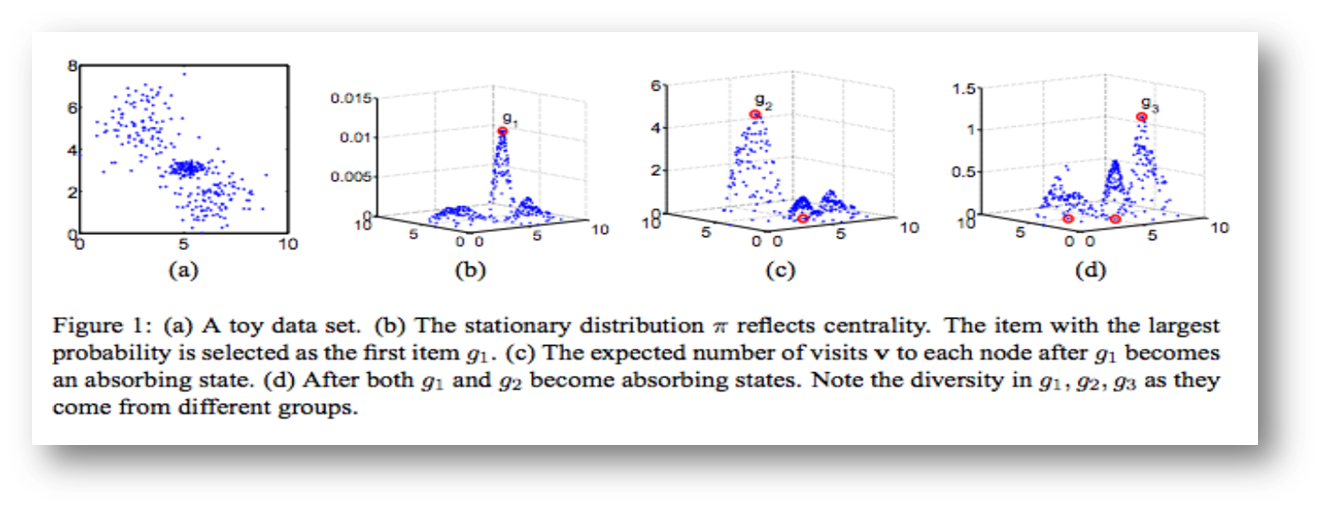
\includegraphics[scale=0.4]{grasshopper}
\caption{Grasshopper on Toy Example.}
\label{fig:grasshopper}
\end{figure}

However, we now have what is termed an absorbing Markov Chain. That is, for the states that are absorbing, we modify $\hat{P}$ such that
\begin{align*}
\hat{P}_{ii} &= 1
\hat{P}_{ij} &= 0 \tag{$i \neq j$}
\end{align*}
for each absorbed state $i$. \\

How do we select the subsequent states? We take a look at the \textit{fundamental matrix} of the absorbing Markov Chain, defined as:
$$
N = (I - \hat{\hat{P}})^{-1}
$$
Note that the vector:
$$
N 1
$$
where $1$ is a vector of $1$s answers the question for the number of steps it takes before entering an absorbing state if we begin at state $i$, by looking at each element $i$. This is how we select the subsequent sentences for our summary, and we repeat the process until the result is presented


Also pertinent to the discussion is the similarity metric. In our implementation, we use the below similarity metric:
% Similarity Metric
  \begin{equation}
    w_{ij} =
    \begin{cases}
      1, & \text{if}\ \frac{s_{i}^\text{T}s_j}{\|s_i\| \|s_j\|} > 0.1 \\
      0, & \text{otherwise}
    \end{cases}
  \end{equation}


From the above discussion, we can derive the pseudo code for our algorithm:

\begin{algorithm}
  \begin{algorithmic}
    \Procedure{GrassHopper}{$D, k, \lambda$} //Where D is a set of documents
    \State{$G \gets BuildMatrix(D)$} // Build the similarity matrix as explained above
    \State{$r \gets initializeDist(\alpha)$} // Create the prior distribution
    \State{$\hat{P} \gets \lambda P + (1-\lambda) r$}
    \State{$stationary \gets getStationary(\hat{P}$}
    \State{$state = np.argmax(stationary)$}
    \State{$Selected \gets [state] $}
    \While{$Selected.len < k$}
      \State{$N \gets fundamental(\hat{P}, selected)$}
        \State{$counts \gets expectedVisists(N)$}
        \State{$max \gets argmax(counts)$}
        \State{$Selected \gets Selected + [max]$}
    \EndWhile{}
    \EndProcedure{}
  \end{algorithmic}
  \caption{Pseudocode for GrassHopper Algorithm.}
\end{algorithm}


\subsection{Modified GrassHopper}
While the above algorithm yields some good results, as shown in our results section, we nonetheless attempted some modifications. We leave most of these for future work, but we propose creating a markov chain as in the GrassHopper algorithm and rather than converting each state into an absorbing state, we make it ``less'' important by adding a uniform transition probability to all output states. In this scenario, we expect the results to improve (though this has not shown to be the case).

\subsection{Modified TextRank}
One issue with TextRank is that it doesn't have a built in mechanism to avoid choosing similar summary sentences. Taking inspiration from GrassHopper, we decided to implement a modified version of TextRank where after running the original TextRank algorithm we add the sentence with the highest score to the summary and all words in the sentence to a set of summary words. Then we reconstruct the Graph, ignoring summary words when creating edges, rerun TextRank and take the sentence with the new highest score. This process is repeated until we extract k sentences. The intent is that on subsequent iterations scores of sentences similar to those in the summary will decrease, leading to broader topic diversity. Due to time constrains we were unable to implement a diversity metric (see future work section).

\section{Experiments}
We now present a thorough analysis of our results, and critiques of our algorithms and our implementations. We also provide details on the data we used for evaluation our system ,and also illustrate some major features. In general, we've learned three major things from implementing this system:
\begin{itemize}
\item Collaboration is more difficult than you expect, and clearly defining and abstracting APIs is non only reasonable but absolutely required.
\item Most algorithms presented in other papers offer little in the help of actually implementing their algorithms. In our case, we buck the trend and release the code openly to anyone who wishes to use it.
\item Evaluation metrics for summaries are currently severely lacking and require significant improvement.
\end{itemize}

Furthermore, we learn that while having good ideas is beneficial, it's always better to have a good system for evaluating them. While we decided to use ROUGE as it appears to be the industry standard, it's surprising to note that the results we achieve are less than stellar. In particular, this is surprising because our summaries appear to be much better, from a human readability perspective. \\

For example, below is an excerpt summary from a human evaluator.
\begin{lstlisting}[breaklines]
Prospects were dim for resolution of the political crisis in Cambodia in October 1998.
Prime Minister Hun Sen insisted that talks take place in Cambodia while opposition leaders Ranariddh and Sam Rainsy, fearing arrest at home, wanted them abroad.
King Sihanouk declined to chair talks in either place.
A U.S. House resolution criticized Hun Sen's regime while the opposition tried to cut off his access to loans.
But in November the King announced a coalition government with Hun Sen heading the executive and Ranariddh leading the parliament.
Left out, Sam Rainsy sought the King's assurance of Hun Sen's promise of safety and freedom for all politicians.
\end{lstlisting}

And now we show the results obtained from our best performing baselines, Frequency:
\begin{lstlisting}[breaklines]
Government and opposition parties have asked King Norodom Sihanouk to host a summit meeting after a series of post-election negotiations between the two opposition groups and Hun Sen's party to form a new government failed.
Hun Sen, however, rejected that.
Both Ranariddh and Sam Rainsy have been outside the country since parliament was ceremonially opened on Sep. 24.
The two parties said that the assembly would convene again Nov. 25.
The prince fled Cambodia and did not return until a few months before elections in July.
\end{lstlisting}

And the results obtained from TextRank:
\begin{lstlisting}[breaklines]
Cambodian leader Hun Sen on Friday rejected opposition parties' demands for talks outside the country, accusing them of trying to ``internationalize'' the political crisis.
Government and opposition parties have asked King Norodom Sihanouk to host a summit meeting after a series of post-election negotiations between the two opposition groups and Hun Sen's party to form a new government failed.
Opposition leaders Prince Norodom Ranariddh and Sam Rainsy, citing Hun Sen's threats to arrest opposition figures after two alleged attempts on his life, said they could not negotiate freely in Cambodia and called for talks at Sihanouk's residence in Beijing.
``I woul
\end{lstlisting}

as well as the results obtained from GrassHopper:
\begin{lstlisting}[breaklines]
Cambodia's two-party opposition asked the Asian Development Bank Monday to stop providing loans to the incumbent government, which it calls illegal.
In a short letter sent to news agencies, the king said he had received copies of cooperation agreements signed Monday that will place Hun Sen and his Cambodian People's Party in firm control of fiscal and administrative functions in the government.
King Norodom Sihanouk on Tuesday praised agreements by Cambodia's top two political parties _ previously bitter rivals _ to form a coalition government led by strongman Hun Sen.
Hun Sen's party recently called on Ranariddh to return to the negotiation table and said
\end{lstlisting}


Qualitatively speaking, the results above show that our system appears to more closely match that of the human summarizer. While the above is simply one example, the code and data are freely available for testing and we're confident when we claim that our summarizer exceeds other current methods, and in particular, performs much better than our baselines from a qualitative point of view.

However, we've also learned that systems for extravtive text summarization are inherently and severely limited. Even in the papers we read, the ROUGE results presented above the baselines are rather minimal and subsequently do not come close to matching the human results.

\subsection{Methods and Models}
We now present the methods we used for evaluation of our data. In our repository, the data from the DUC 2004 competitions can be found, as well as the data used for this system. For more information, see the \verb|README.md| in the respository or the Appendix section of this paper.

The documents themselves were pre-processed to allow for each document to consists of a sequences of sentences separated by newlines. The DUC 2004 Task 2 documents are then read by our system and split into sentences based on this expected input syntax. Subsequently,
\begin{enumerate}
\item We split into sentences using the NLTK Punkt splitter (with default settings)
\item We then parse each word. Note that sentences are represented as a vector of words, rather than as a single string.
\item Each word in the sentence is stemmed using the Porter Stemmer from the NLTK library.
\item After stemming and cleaning, all words are lower-cased.
\item The text is then processed and converted into the vector representations as required by each algorithm.
\item Most vector representations that rely on a count of words, lowercase the input word before processing so we don't capture any information on capitalization.
\end{enumerate}

Once the above has been accomplished for each document, the processed document set is fed to each summarizaton algorithm, which is tasked with returning the appropriate summary. We then post-process the summary:
\begin{enumerate}
\item If asked to, we truncate the input to the specified number of bytes. This is true by default, so most output
\item If asked to, the system then runs ROUGE on the output summary files and compares them to the model files (see \verb|--help| for more information).
\item Note that ROUGE runs with the following, parameters, stolen from the DUC 2007 conference.
\begin{verbatim}
-b -1 -c 95 -n 4 -w 1.2 -a -f A -p 0.5 -t 0 -m
\end{verbatim}
\end{enumerate}

\subsection{Results}
Table \ref{tab:results} gives the resulting average ROUGE-1 and ROUGE-2 Recall scores for each of the algorithms run on the data from DUC 2004 task 2. In addition to the summaries produced by the implemented algorithms we also have average scores summaries from one of the human summarizers used to evaluate results for the conference. To be honest, we're quite baffled with the results, as our novel Word Freqs baseline seemingly outperformed the Human Summaries (to be consistent with DUC 2004 evaluation, we truncated all summaries at 665 bytes). While this would have been encouraging if the resulting summaries were of high quality, they mainly consist of short choppy sentences, some of which could almost pass for poetry (see below).

\begin{verbatim}
His career is on the line.
It's just ugly.
So did McCain.
And Newt knows it.
The big picture.
\end{verbatim}

Looking through the algorithm generated summaries and the human ones they were scored against, we don't understand how the Word Freqs summaries are getting such high scores (the high scores from the conference were below 0.4 which our naive baselines are seemingly blowing out of the water despite being run on what we believe to be the same documents and model summaries). This makes us a bit skeptical about whether ROUGE is working correctly. If somehow ROUGE is working correctly, we're definitely disappointed with the performance of TextRank and GrassHopper, as they performed worse or barely edged out our simple baselines. (@Sasha if you're curious about why we're getting strange rouge scores and want to follow up to take a look let us know :) )

\begin{table}[]
\centering
\caption{Resulting Rouge-1 and Rouge-2 Recall Scores}
\label{tab:results}
\resizebox{\textwidth}{!}{
\begin{tabular}{lcccc}
\textbf{Algorithm} & \multicolumn{1}{l}{\textbf{Average Rouge-1\_R Score}} & \textbf{Roude-1\_R: 95\% CI} & \multicolumn{1}{l}{\textbf{Average Rouge-2\_R Score}} & \textbf{Rouge-2\_R: 95\% CI} \\
Naive Baseline & .5342 & 0.5198 - 0.5494 & 0.3704 & 0.3564 - 0.3843 \\
Word Freqs & 0.6073 & 0.5967 - 0.6175 & 0.4433 & 0.4343 - 0.4527 \\
Geom Prior & 0.5478 & 0.5369 - 0.5575 & 0.3846 & 0.3731 - 0.3957 \\
Modified Geom Prior & 0.5444 & 0.5316 - 0.5570 & 0.3834 & 0.3723 - 0.3948 \\
Multiple Geom Prior & 0.5374 & 0.5249 - 0.5494 & 0.3780 & 0.3673 - 0.3920 \\
TextRank & 0.5373 & 0.5230 - 0.5523 & 0.3693 & 0.35660 - 0.3823 \\
Modified TextRank & 0.5220 & 0.4975 - 0.5485 & 0.3597 & 0.3336 - 0.3843 \\
GrassHopper & 0.5287 & 0.5159 - 0.5409 & 0.3620 & 0.3487 - 0.3742 \\
Modified GrassHopper & 0.5173 & 0.5023 - 0.5323 & 0.3539 & 0.3399 - 0.3677 \\
\begin{tabular}[c]{@{}l@{}}Human Summary  (From \\ DUC evaluation data)\end{tabular} & 0.6002 & 0.5802 - 0.6180 & 0.4226 & 0.4053 - 0.4392
\end{tabular}}
\end{table}

\subsection{Discussion}
As we can see from the results above, the results from our extractive summarization library appear to be objectively less than stellar. However, qualitatively gauging the summaries produced, we feel like our library and modified algorithms do an adequate job and are likely on par with others out there. Additionally, we've made an effort to make our data as open as possible, as well as our code, because we found it extremely difficult reading papers which discussed algorithms, presented results, but then had no way to verify their results. Even if we wanted to, some papers made it extremely difficult to access the data they used for testing. We make an effort to do the opposite by being as transparent as possible with our results and data.

We originally decided to take on this project because neither of us had done any NLP work and we thought it would be a good learning opportunity. We found the course material to be engaging, and felt something like this would be a natural extension of the material we learned from Finale and others on machine learning. In tackling this project we've learned that, among other things, text summarization is really hard. We thought extractive summarization was a relatively simple idea, but from our own work and the papers we've read it seems that doing substantially better than the first sentence of every paragraph is not a trivial task. Rather than using our extractive summaries to replace reading an article, we think extractive summarization has potential as a great study tool-imagine being able to automatically highlight key ideas in your gen ed reading!

\section{Future Work}
While we were able to beat our baseline models, there is a lot of room for improvement. Right now the similarity functions used to create our graphs do not account for the fact that words can be synonyms, so we think doing so would be a straightforward way to improve the performance of our implementations of TextRank and GrassHopper. We are also curious about the effects of using different similarity functions such as log-TF, TF-IDF, etc. to determine edges and weights in the algorithms. Additionally we'd like to use the spearmint package for Bayesian optimization to tune our parameters. \\
In addition to ways for improving our algorithms themselves, we're interested in different methods for evaluating our results. This includes alternatives to ROUGE for measuring summary quality, and a way to measure summary diversity. One naive measure of diversity we came up with was to score words based on frequency the way we did in our Word Frequency baseline, and score a summary's diversity as the sum of the word scores of the union of it's sentences. While it's certainly a naive measure (there are papers with much more sophisticated approaches), it's one we could implement relatively quickly to get a feel for if GrassHopper is actually picking up different a broader set of ideas than TextRank, or if our modification to TextRank actually helped in this regard. As for an alternative to ROUGE, our grievances were voiced in the discussion section above.

\appendix

\section{Program Trace}
\label{sec:program_trace}

We now present a trace of the program as it summarizes a single document set utilizing the {\sc GrassHopper} algorithm with our own modification. We present an abbreviated version of the traceback. Note that we have included a tool, \verb|tracer.py| which allows for the generation of traces. Note that without ignoring some modules (such as utils.py), traces can run into the hundreds of megabytes and take a few minutes to generate.

The command, using the above tool which can be found in the root directory of our repository, used to generate the below trace, is now presented. Note that the command is executed from the root directory.
\begin{lstlisting}
python tracer.py --data_dir=sample_rouge_data --algorithm=grasshopper \
  --rouge_score=True --summarize=True --debug=True --bytes=665 > trace.out
\end{lstlisting}
However, if running without rouge, the command should be:
\begin{lstlisting}
python tracer.py --data_dir=sample_rouge_data --algorithm=grasshopper \
  --rouge_score=False --summarize=True --debug=True > trace.out
\end{lstlisting}

If more detail on the trace is required, modifications on \verb|tracer.py| can be made to ignore fewer modules. Note that the trace presented below can be viewed in its entirety \href{https://raw.githubusercontent.com/kandluis/document_summaries/master/trace.out}{here}.
\begin{lstlisting}[breaklines,language=Python]
<string>(1):   --- modulename: summarizer, funcname: run
summarizer.py(129):     base = None if opts.data_dir is None else os.path.abspath(opts.data_dir)
summarizer.py(130):     debug = opts.debug.lower() == 'true'
summarizer.py(131):     bytes = int(opts.bytes)
summarizer.py(132):     sort_sents = opts.sort_sents.lower() == 'true'
summarizer.py(133):     k = int(opts.summary_length)
summarizer.py(135):     if opts.summarize.lower() == 'true':
summarizer.py(136):         try:
summarizer.py(137):             algorithm = argsToAlgo[opts.algorithm.lower()]
summarizer.py(144):     inputParams = "_sorted={}_k={}_bytes={}".format(sort_sents, k, bytes)
summarizer.py(145):     outpath = None if base is None else os.path.join(
summarizer.py(146):         base, opts.algorithm + inputParams)
summarizer.py(147):     if opts.summarize.lower() == 'true':
summarizer.py(148):         if base is None:
summarizer.py(154):         if not os.path.exists(outpath):
summarizer.py(155):             os.makedirs(outpath)
summarizer.py(157):         inbase = os.path.join(base, 'docs')
summarizer.py(158):         folders = dirs = [d for d in os.listdir(
summarizer.py(159):             inbase) if os.path.isdir(os.path.join(inbase, d))]
 --- modulename: stat, funcname: S_ISDIR
stat.py(41):     return S_IFMT(mode) == S_IFDIR
 --- modulename: stat, funcname: S_IFMT
stat.py(25):     return mode & 0170000
summarizer.py(159):             inbase) if os.path.isdir(os.path.join(inbase, d))]
summarizer.py(160):         for folder in folders:
summarizer.py(161):             inpath = os.path.join(inbase, folder)
summarizer.py(162):             try:
summarizer.py(163):                 createSummaries(algorithm, inpath, outpath, sort_sents, bytes=bytes,
summarizer.py(164):                                 k=k, multiDocument=True)
 --- modulename: summarizer, funcname: createSummaries
summarizer.py(87):     setID = abs_path.split('/')[-1]
summarizer.py(90):     docIDs = []
summarizer.py(93):     D = []
summarizer.py(94):     for filename in os.listdir(abs_path):
summarizer.py(96):         tmp = filename.split('.')
summarizer.py(97):         if tmp[0] == 'Parsed':
summarizer.py(98):             docIDs.append(tmp[1])
summarizer.py(99):             filepath = os.path.join(abs_path, filename)
summarizer.py(100):             with open(filepath) as inputDoc:
summarizer.py(101):                 text = inputDoc.read().strip()
summarizer.py(102):                 sentences = tokenizer.tokenize(text)
summarizer.py(103):                 D.append([s.split(" ") for s in sentences])
summarizer.py(103):                 D.append([s.split(" ") for s in sentences])
summarizer.py(103):                 D.append([s.split(" ") for s in sentences])
summarizer.py(103):                 D.append([s.split(" ") for s in sentences])
summarizer.py(103):                 D.append([s.split(" ") for s in sentences])
summarizer.py(103):                 D.append([s.split(" ") for s in sentences])
summarizer.py(103):                 D.append([s.split(" ") for s in sentences])
summarizer.py(103):                 D.append([s.split(" ") for s in sentences])
summarizer.py(103):                 D.append([s.split(" ") for s in sentences])
summarizer.py(103):                 D.append([s.split(" ") for s in sentences])
summarizer.py(103):                 D.append([s.split(" ") for s in sentences])
summarizer.py(103):                 D.append([s.split(" ") for s in sentences])
summarizer.py(103):                 D.append([s.split(" ") for s in sentences])
summarizer.py(103):                 D.append([s.split(" ") for s in sentences])
summarizer.py(103):                 D.append([s.split(" ") for s in sentences])
summarizer.py(103):                 D.append([s.split(" ") for s in sentences])
summarizer.py(103):                 D.append([s.split(" ") for s in sentences])
...
grasshopper.py(220):     D = [s for d in D for s in d]
grasshopper.py(220):     D = [s for d in D for s in d]
grasshopper.py(220):     D = [s for d in D for s in d]
grasshopper.py(220):     D = [s for d in D for s in d]
grasshopper.py(220):     D = [s for d in D for s in d]
grasshopper.py(220):     D = [s for d in D for s in d]
grasshopper.py(220):     D = [s for d in D for s in d]
grasshopper.py(220):     D = [s for d in D for s in d]
...
grasshopper.py(223):     cleanDoc, mapping = utils.cleanDocument(D)
grasshopper.py(224):     WClean = docToMatrix(
grasshopper.py(225):         cleanDoc, sim_fun=utils.threshHoldCosineSim)
 --- modulename: grasshopper, funcname: docToMatrix
grasshopper.py(80):     sentenceVectors = vec_fun(D)
grasshopper.py(83):     n = len(D)
grasshopper.py(84):     M = np.zeros((n, n))
grasshopper.py(85):     for i in range(n):
grasshopper.py(86):         for j in range(n):
grasshopper.py(87):             M[i, j] = sim_fun(sentenceVectors[i], sentenceVectors[j])
 --- modulename: _abcoll, funcname: __subclasshook__
_abcoll.py(100):         if cls is Sized:
_abcoll.py(103):         return NotImplemented
 --- modulename: _abcoll, funcname: __subclasshook__
_abcoll.py(100):         if cls is Sized:
_abcoll.py(103):         return NotImplemented
grasshopper.py(86):         for j in range(n):
grasshopper.py(87):             M[i, j] = sim_fun(sentenceVectors[i], sentenceVectors[j])
grasshopper.py(86):         for j in range(n):
grasshopper.py(87):             M[i, j] = sim_fun(sentenceVectors[i], sentenceVectors[j])
grasshopper.py(86):         for j in range(n):
grasshopper.py(87):             M[i, j] = sim_fun(sentenceVectors[i], sentenceVectors[j])
grasshopper.py(86):         for j in range(n):
grasshopper.py(87):             M[i, j] = sim_fun(sentenceVectors[i], sentenceVectors[j])
grasshopper.py(86):         for j in range(n):
grasshopper.py(87):             M[i, j] = sim_fun(sentenceVectors[i], sentenceVectors[j])
grasshopper.py(86):         for j in range(n):
...
grasshopper.py(87):             M[i, j] = sim_fun(sentenceVectors[i], sentenceVectors[j])
grasshopper.py(86):         for j in range(n):
grasshopper.py(85):     for i in range(n):
grasshopper.py(88):     return M
grasshopper.py(229):     lamb = 0.5
grasshopper.py(230):     alpha = 0.25
grasshopper.py(231):     r = utils.decayDistribution(alpha, len(WClean))
grasshopper.py(232):     summary = algo(WClean, r, lamb, k)
 --- modulename: grasshopper, funcname: grasshopper
grasshopper.py(118):     n, m = W.shape
grasshopper.py(119):     assert n == m  # Sizes should be equal
grasshopper.py(120):     assert np.min(W) >= 0  # No negative edges
grasshopper.py(121):     assert abs(np.sum(r) - 1) < epsilon  # r is a distribution
grasshopper.py(122):     assert 0 <= lamb and lamb <= 1  # lambda is valid
grasshopper.py(123):     assert 0 < k and k <= n  # Summary can't be longer than document!
grasshopper.py(126):     P = W / np.sum(W, axis=1)
grasshopper.py(127):     r = r.reshape((1, len(P)))
grasshopper.py(128):     hatP = lamb * P + (1 - lamb) * r
grasshopper.py(130):     assert hatP.shape == (n, m)  # Shape should not change!
grasshopper.py(133):     absorbed = []
grasshopper.py(134):     nonAbsorbed = range(n)
grasshopper.py(135):     probs = []
grasshopper.py(138):     q = stationary(hatP)
 --- modulename: grasshopper, funcname: stationary
grasshopper.py(25):     values, vectors = np.linalg.eig(Mat.T)
 --- modulename: numeric, funcname: asarray
numeric.py(474):     return array(a, dtype, copy=False, order=order)
 --- modulename: numeric, funcname: asanyarray
numeric.py(525):     return array(a, dtype, copy=False, order=order, subok=True)
grasshopper.py(26):     index = np.nonzero(abs(values - 1.) < epsilon)[0][0]
grasshopper.py(28):     q = np.real(vectors[:, index])
 --- modulename: type_check, funcname: real
type_check.py(139):     return asanyarray(val).real
 --- modulename: numeric, funcname: asanyarray
numeric.py(525):     return array(a, dtype, copy=False, order=order, subok=True)
grasshopper.py(29):     assert(abs((q**2).sum() - 1) < epsilon)
grasshopper.py(31):     return q / np.sum(q)  # convert into probability distribution
grasshopper.py(139):     maxState = np.argmax(q)
grasshopper.py(140):     absorbed.append(maxState)
grasshopper.py(141):     probs.append(np.max(q))
grasshopper.py(142):     nonAbsorbed.remove(maxState)
grasshopper.py(146):     while (len(absorbed) < k):
grasshopper.py(151):         N = np.linalg.inv(
grasshopper.py(152):             np.identity(len(nonAbsorbed)) - hatP[nonAbsorbed, nonAbsorbed])
 --- modulename: numeric, funcname: identity
numeric.py(2209):     from numpy import eye
numeric.py(2210):     return eye(n, dtype=dtype)
 --- modulename: numeric, funcname: asarray
numeric.py(474):     return array(a, dtype, copy=False, order=order)
grasshopper.py(155):         nuvisit = np.sum(N, axis=0)
grasshopper.py(156):         nvisit = np.zeros(n)
grasshopper.py(157):         nvisit[nonAbsorbed] = nuvisit
grasshopper.py(160):         absorbState = np.argmax(nvisit)
grasshopper.py(161):         absorbVisit = max(nvisit)
grasshopper.py(163):         absorbed.append(absorbState)
grasshopper.py(164):         probs.append(absorbVisit)
grasshopper.py(166):         nonAbsorbed.remove(absorbState)
grasshopper.py(146):     while (len(absorbed) < k):
grasshopper.py(151):         N = np.linalg.inv(
grasshopper.py(152):             np.identity(len(nonAbsorbed)) - hatP[nonAbsorbed, nonAbsorbed])
 --- modulename: numeric, funcname: identity
numeric.py(2209):     from numpy import eye
numeric.py(2210):     return eye(n, dtype=dtype)
 --- modulename: numeric, funcname: asarray
numeric.py(474):     return array(a, dtype, copy=False, order=order)
grasshopper.py(155):         nuvisit = np.sum(N, axis=0)
grasshopper.py(156):         nvisit = np.zeros(n)
grasshopper.py(157):         nvisit[nonAbsorbed] = nuvisit
grasshopper.py(160):         absorbState = np.argmax(nvisit)
grasshopper.py(161):         absorbVisit = max(nvisit)
grasshopper.py(163):         absorbed.append(absorbState)
grasshopper.py(164):         probs.append(absorbVisit)
grasshopper.py(166):         nonAbsorbed.remove(absorbState)
grasshopper.py(146):     while (len(absorbed) < k):
grasshopper.py(151):         N = np.linalg.inv(
grasshopper.py(152):             np.identity(len(nonAbsorbed)) - hatP[nonAbsorbed, nonAbsorbed])
 --- modulename: numeric, funcname: identity
numeric.py(2209):     from numpy import eye
numeric.py(2210):     return eye(n, dtype=dtype)
 --- modulename: numeric, funcname: asarray
numeric.py(474):     return array(a, dtype, copy=False, order=order)
grasshopper.py(155):         nuvisit = np.sum(N, axis=0)
grasshopper.py(156):         nvisit = np.zeros(n)
grasshopper.py(157):         nvisit[nonAbsorbed] = nuvisit
grasshopper.py(160):         absorbState = np.argmax(nvisit)
grasshopper.py(161):         absorbVisit = max(nvisit)
grasshopper.py(163):         absorbed.append(absorbState)
grasshopper.py(164):         probs.append(absorbVisit)
grasshopper.py(166):         nonAbsorbed.remove(absorbState)
grasshopper.py(146):     while (len(absorbed) < k):
grasshopper.py(151):         N = np.linalg.inv(
grasshopper.py(152):             np.identity(len(nonAbsorbed)) - hatP[nonAbsorbed, nonAbsorbed])
 --- modulename: numeric, funcname: identity
numeric.py(2209):     from numpy import eye
numeric.py(2210):     return eye(n, dtype=dtype)
 --- modulename: numeric, funcname: asarray
numeric.py(474):     return array(a, dtype, copy=False, order=order)
grasshopper.py(155):         nuvisit = np.sum(N, axis=0)
grasshopper.py(156):         nvisit = np.zeros(n)
grasshopper.py(157):         nvisit[nonAbsorbed] = nuvisit
grasshopper.py(160):         absorbState = np.argmax(nvisit)
grasshopper.py(161):         absorbVisit = max(nvisit)
grasshopper.py(163):         absorbed.append(absorbState)
grasshopper.py(164):         probs.append(absorbVisit)
grasshopper.py(166):         nonAbsorbed.remove(absorbState)
grasshopper.py(146):     while (len(absorbed) < k):
grasshopper.py(169):     return absorbed
grasshopper.py(234):     return summary, D, mapping
 --- modulename: summarizer, funcname: processSummary
summarizer.py(80):     if sort_sents:
summarizer.py(81):         sentences = sorted(sentences)
summarizer.py(82):     return [D[mapping[i]] for i in sentences]
summarizer.py(82):     return [D[mapping[i]] for i in sentences]
summarizer.py(82):     return [D[mapping[i]] for i in sentences]
summarizer.py(82):     return [D[mapping[i]] for i in sentences]
summarizer.py(82):     return [D[mapping[i]] for i in sentences]
summarizer.py(82):     return [D[mapping[i]] for i in sentences]
summarizer.py(111):         filepath = os.path.join(out_path, "SetSummary.{}.txt".format(setID))
summarizer.py(112):         with open(filepath, 'w+') as out:
summarizer.py(113):             res = "\n".join([" ".join(s).strip() for s in summary])
summarizer.py(113):             res = "\n".join([" ".join(s).strip() for s in summary])
summarizer.py(113):             res = "\n".join([" ".join(s).strip() for s in summary])
summarizer.py(113):             res = "\n".join([" ".join(s).strip() for s in summary])
summarizer.py(113):             res = "\n".join([" ".join(s).strip() for s in summary])
summarizer.py(113):             res = "\n".join([" ".join(s).strip() for s in summary])
summarizer.py(114):             out.write(res[:bytes])
summarizer.py(160):         for folder in folders:
summarizer.py(172):     if base is not None and opts.rouge_score == 'True':
 --- modulename: trace, funcname: _unsettrace
trace.py(80):         sys.settrace(None)
\end{lstlisting}

For other tracebacks, we provide the results. Note that the syntax for the provided \verb|tracer.py| program

\section{System Description}
For a more detailed description of how to run our system, please take a look at the README.md file in the \href{https://github.com/kandluis/document_summaries}{github repository}. Note that for a short summary of what's presented below, the \verb|--help| flag will be handy.

\subsection{DUC 2004 Sample Data}
\label{subsec:duc_sample_data}
We now provided a short description on how to generate some of the sample summaries presented in the text, which are included in the github repository. Note that the commands presented below should be runnable directly as soon as the repository is cloned and a the appropriate requirements fulfilled.

\begin{enumerate}
\item Clone the github repository using
\begin{lstlisting}[language=Python, caption="Git Clone Command"]
git clone git@github.com:kandluis/document_summaries.git
\end{lstlisting}
\item See \verb|README.md| for details on the required packages. At minimum,
\begin{enumerate}
\item Install \href{http://www.nltk.org/}{NLTK}
\item Install \href{http://www.numpy.org/}{numpy}
\end{enumerate}
\item The trace described in Appendix \ref{sec:program_trace} can be executed with the command:
\begin{lstlisting} [breaklines]
python tracer.py --data_dir=sample_rouge_data --algorithm=grasshopper --rouge_score=True --summarize=True --debug=True > trace.out
\end{lstlisting}
\item For other sample commands, the general format, after installation:
\begin{lstlisting}[breaklines]
python -m summarizer --data_dir=sample_rouge_data --algorithm=ALGORITHM --summarize=True --rouge_score=False --debug=True --summary_length=5
\end{lstlisting}
The above command, with the appropriate substitution of \verb|ALGORITHM| with one of \{GrassHopper,  FirstGeomPrior, Baseline, GeomPrior, Frequency, TextRank \}. The command will take the input sample data contained in the \verb|sameple_rouge_data/docs/| directory \footnote{As of the time of the writing of this paper, the data contained consists of a single collection from the DUC 2004 Task 1/2 data set. The set selected consists of ID 30001.}
\end{enumerate}
For more assistance on how to run the program, see the \verb|README.md| or run the summarizer with the \verb|--help| flag to receive more details \footnote{Note that the system attempts to generate, by default, summaries containing 665 characters.}.

As per the \verb|README.md|, note that it is further possible to verify the presented results by running the system directly, with new summaries, and calculating the ROUGE scores in comparison to the model summaries \footnote{The model summaries are obtained from the DUC 2003 conference. They can also be found directly here:\href{https://www.dropbox.com/sh/dzmzh5nwe1i68ra/AABYPkOj6lXZln5I6tEDjpAna?dl=0}{https://www.dropbox.com/sh/dzmzh5nwe1i68ra/AABYPkOj6lXZln5I6tEDjpAna?dl=0}}. While we do not recommend taking this approach, due to the level of difficulty,

\subsection{Standard Input}
\label{subsec:standard_input}
An alternative method for running the system which does not require initial data consists of summarizing single documents through the use of the commandline interface itself. Suppose we have the following in a text file \verb|sample.txt|:
\begin{lstlisting}[breaklines]
Use short sentences to create punch and make a point.
Use phrases and even words as sentences. Really.
Do not use too many sentences -- about three or four is usually enough.
Use a short sentence as a summary after a longer description.
Generally speaking, a short sentence works well at the start of a paragraph or speech item to grab attention, and at the end, to summarize and signal completion.
\end{lstlisting}
We can create a simple 1-sentence summary with the command:
\begin{lstlisting}[breaklines]
python -m summarizer --algorithm=ALGORITHM --rouge_score=False --summarize=True --debug=True -k 1 < sample.txt
\end{lstlisting}
We present the results of the above command for each for the algorithms:
\begin{enumerate}
\item {\sc Baseline}: Use short sentences to create punch and make a point.
\item {\sc GeomPrior}: Generally speaking, a short sentence works well at the start of a paragraph or speech item to grab attention, and at the end, to summarize and signal completion. \footnote{Not deterministic.}
\item {\sc FirstGeomPrior}: Use short sentences to create punch and make a point.
\item {\sc Frequency}: Use short sentences to create punch and make a point.
\item {\sc Grasshopper }: Use short sentences to create punch and make a point.
\item {\sc TextRank}: Generally speaking, a short sentence works well at the start of a paragraph or speech item to grab attention, and at the end, to summarize and signal completion.
\end{enumerate}
Note, however, that the system does not provide an evaluation for the quality of the score under these circumstances. In order to receive ROUGE metric, the system must be run with as described in Append \ref{subsec:duc_sample_data}.

\section{Group Makeup}
Our project groups consists of two individuals, Kevin Eskici and Luis A. Perez. The work was divided fairly evenly, and as described in our original proposal, with no major modifications. In detail, we have the below:
\begin{enumerate}
\item Luis Antonio Perez. The tasks are listed in order of importance/difficulty.
\begin{itemize}
\item Main Task: Understand and implement the {\sc GrassHopper} as described by Zhu et al. \cite{grasshopper}.
\item Explore the parameter space for {\sc GrassHopper} and optimize the parameters on the DUC 2004 data using ROUGE as a sample metric.
\item Improve upon basic implementation of the baselines, and incorporate the results into the general framework.
\item Understand ROUGE and ROUGE scores \cite{rouge}.
\item Generate a general framework for testing our differing algorithms with the use of ROUGE.
\item Generalize framework and add options for easy of use.
\item Create a usable, testable system, which involves writing code to clean and parse the original data automatically, as well as code to help with structuring the overall layout of the project.
\end{itemize}
\item Kevin Eskici
\begin{itemize}
\item Main Task: Understand and implement the {\sc TextRank} algorithm, as described by Mihalcea et al \cite{textrank}.
\item Explore the parameter space for {\sc TextRank} and implement modifications to the algorithm with the purpose of increasing diversity, if possible.
\item Implement the baselines, including multiple naive baselines as well as more clever baselines which attempt to assign score to sentences.
\item Improve upon baselines by exploring different priors over the distributions.
\item Explore NLTK corpus and DUC corpus for relevant information and metrics.
\item Include explorations and testing framework from NLTK
\item Help with sentence partitioning and sentence detection, as well as word tagging as required by the TextRank algorithm.
\end{itemize}
\end{enumerate}
The code for the project is completely open source and can be found on \href{https://github.com/kandluis/document_summaries}{github}. Requests for access to the processed data summaries for DUC 2004 can be sent to \href{mailto:luis.perez.live@gmail.com}{luis.perez.live@gmail.com}. For direct access to the data, please see \href{https://www.dropbox.com/sh/dzmzh5nwe1i68ra/AABYPkOj6lXZln5I6tEDjpAna?dl=0}{here}.

\bibliographystyle{plain}
\bibliography{references}

\end{document}
